\documentclass[a4paper,12pt,]{article}
\usepackage[utf8]{inputenc}

\title{Feature 4: Sensibilisierung für Nachhaltigkeit am Arbeitsplatz}
\author{A.~Heckl, A.~Kohles, A.~Lehene, A.~Mütter}
\date{Februar 2020}

\usepackage[left=2.5cm,right=2.5cm,top=2.5cm,bottom=2.5cm]{geometry}
\usepackage{natbib}
\usepackage{graphicx}
\usepackage[ngerman]{babel}
\newcommand{\ToDo}[1]{
\begin{center}
\fbox{
\begin{minipage}{0.9\textwidth}
#1
\end{minipage}
}
\end{center}
}

\begin{document}

\maketitle
\begin{figure}
\begin{minipage}[b]{\textwidth}
\ToDo{\tiny\textbf{Hinweis:} Wir waren uns bei der Formulierung des Tagebuchs und des Abschlussberichts über die Richtlinien der gendergerechten Sprache und der gendergerechten Formulierung bewusst.
Aus Gründen der Übersichtlichkeit und der einfacheren Lesbarkeit haben wir uns entschieden darauf hinzuweisen, dass in diesem Dokument mit allen männlichen Formulierungen von Personen (Angestellter, Mitarbeiter, Vorgesetzter) selbstverständlich auch die weiblichen Pendants gemeint sind, und diese in keiner Weise vernachlässigbar oder weniger bedeutungsvoll sind.}
\end{minipage}
\end{figure}

\section{Deskriptive Systembeschreibung}

Es gibt einen anhaltenden Trend zu Nachhaltigkeit und Umweltschutz.
Arbeitgeber möchten ihre Mitarbeiter für diese Themen sensibilisieren, um
einerseits an Materialkosten einzusparen und andererseits
Materialverschwendung einzudämmen. Darüber hinaus soll vor allem das
Image des Unternehmens „grüner“ werden. Mitarbeiter sollen angeregt
werden für ihre Heißgetränke vermehrt eigene Tassen und
Mehrwegbecher, anstatt von Papp- und Plastikbechern zu benutzen. Dies
soll erreicht werden, indem die Getränkemaschine für jeden Mitarbeiter
bei der Zubereitung eines Getränks die verwendete Art von Behälter
(Einweg oder Mehrweg) aufzeichnet, sowie ob das gekaufte Getränk über
ein Bio-Siegel verfügt oder nicht. Alle gesammelten Daten werden
wöchentlich als CSV-Datei bereitgestellt. Auf Basis dieser Dateien sollen
die Mitarbeiter persönlich analysiert werden. Dies erfolgt zum einen durch
Verlaufskurven, die Einweg- und Mehrwegbecherbenutzung aufzeigen,
zum anderen durch Vergleich der Mitarbeiter in Form von Rankings. Sogar
ein Belohnungssystem auf Basis dieser Rankings ist vorstellbar.

Bei dieser Art von Gadget ist neben dem Arbeitgeber und den
Arbeitnehmern auch die PR-Abteilung des Unternehmens involviert.

\section{Wertekonflikte}

\subsection{Fragestellungen}
Vor der Umsetzung einer solchen Maßnahme gibt es jedoch
aufkommende Fragestellungen:
\begin{itemize}
\item
Ist es überhaupt sinnvoll oder vertretbar Mitarbeiter als
Umweltsünder darzustellen?
\item
Wird eine Spaltung der Mitarbeiter in Umweltsünder und
Umweltschützer erfolgen?

\item
Wer darf die von der Kaffeemaschine aufgezeichneten Daten
überhaupt einsehen?

\item
Darf man Mitarbeiter aufgrund ihrer ausgewählten Becher
ranken und evtl. sogar bestrafen oder belohnen?

\item
Dürfen Arbeitgeber das Konsumverhalten ihrer Mitarbeiter
überwachen? Dürfen Arbeitgeber sich in das private Thema
Nachhaltigkeit einmischen?

\item
Ist eine solche Maßnahme überhaupt sinnvoll oder ist der
Einfluss auf Umweltverschmutzung bzw. Klimawandel
verschwindend gering?
\end{itemize}

\subsection{Biases}
Zunächst sollte man sich mit den sogenannten Preexisting
biases auseinandersetzen. Hierzu muss gesagt werden, dass Kaffee eine
produktivitätssteigernde Wirkung (``Anregung des Zentralnervensystems")\footnote{\tt https://www.chemie.de/lexikonKoffein.html$\#$Hauptwirkungen\_des\_Koffeins}
hat und verträglicher als andere Aufputschmittel, wie zum Beispiel Energydrinks\footnote{\tt https://www.welt.de/gesundheit/article145259849/Das-macht-eine-Dose-Red-Bull-mit-
Ihrem-Koerper.html} und im Vergleich zu Drogen wie Kokain legal erhältlich ist.
Auch in Betracht gezogen werden muss, dass das Einsparen von kleinen
Einwegbechern keinen großen Beitrag zum Schutz der Umwelt liefert.
Ferner kann es Mitarbeiter geben, die nicht an den Klimawandel glauben
oder die keinen Beitrag zum Schutz der Natur und Umwelt leisten
möchten und deswegen oder auch aus anderen Gründen keine Änderung
ihres bisherigen Konsumverhaltens vornehmen möchten. Zudem ist die
Umweltverträglichkeit abhängig vom verwendeten Mehrwegutensil.\footnote{\tt https://www.quarks.de/umwelt/muell/nur-so-sind-kaffee-mehrwegbecher-
umweltfreundlich/}
Zusätzlich lassen sich auch Technical biases feststellen: Zunächst
muss man sich im Klaren sein, dass nicht jeder Konsum von
Heißgetränken gemessen werden kann. Von zuhause mitgebrachte oder
von extern gekaufte (z.B Bäckerei neben Firmengelände) Getränke
können in den Auswertungen nicht berücksichtigt werden, sodass das
Ranking der umweltfreundlichsten und umweltfeindlichsten Mitarbeitern
und Mitarbeiterinnen nicht der Realität entsprechen muss sondern sich
lediglich auf die Benutzung der unternehmensinternen
Getränkemaschinen beschränkt. Diese und weitere Gründe, wie zum
Beispiel, dass ein Mitarbeiter einem anderen Mitarbeiter oder einem Gast
Kaffee mitbringt oder ausgibt, können zu Verfälschungen der Daten
führen.
Weiterhin gibt es auch Emergent biases, die für dieses Gadget
aufkommen: Mitarbeiter könnten argumentieren, dass sie nur Einwegbecher verwenden um keine Zeit mit dem Abspülen von Tassen zu
verbrauchen um im Endeffekt produktiver und wertvoller für das
Unternehmen zu sein. Außerdem ist vorstellbar, dass die Mitarbeiter sich
überwacht fühlen und sie sich ihre Heißgetränke verstärkt von anderen
Quellen holen oder gar auf den Konsum dieser verzichten. Beide
Alternativen könnten zu Produktivitätsverlust führen: Die Erste aufgrund
„vergeudeter“ Zeit und die Zweite wegen der fehlenden Energieschübe,
die man durch Koffein bekommt. Hinzu kommt, dass Mitarbeiter als
Protestreaktion auf die Überwachung zunehmend zur Ablehnung von
Umweltschutzmaßnahmen tendieren oder dem Klimawandel skeptischer
gegenüberstehen. Außerdem ist nicht zu unterschätzen, dass Rankings
als Mobbing- oder Erpressungsinstrument missbraucht werden können.

\subsection{Vortheoretische Deliberation}
In Anbetracht der Fragestellungen und verschiedenen Bias, stellt sich
die Frage ob und wie dieses Feature umgesetzt werden soll. Einige
Einschränkungen lassen sich dabei klar erkennen: Die Ergebnisse, die
dieses Gadget liefert, dürfen weder als Druckmittel noch als
Rechtfertigung zu Bestrafungen fungieren. Unter anderem zu diesem
Zweck muss mit den gesammelten Daten vertraulich umgegangen
werden, indem man sie beispielsweise anonymisiert. Da dies einhaltbare
Richtlinien sind erscheint eine Umsetzung des Gadgets zunächst sinnvoll.

\section{Ethische Systemüberprüfung}

Im Folgendem wird die Umsetzung des Features aus verschiedenen
Sichtweisen analysiert: zunächst deontologisch nach Kants kategorischem
Imperativ und anschließend konsequentialistisch nach utilitaristischem
Konzept.

\subsection{Deontologische Betrachtung}

Für die Einführung eines solchen Features lässt sich feststellen, dass es wünschenswert ist, dass alle Menschen umweltbewusst handeln. Somit ist die Umsetzung eines Tools, dass die Mitarbeiter erinnert sich ein klimaneutraleres und umweltschonenderes Verhalten anzugewöhnen, erstrebenswert. Dabei zählt insbesondere, dass jede Handlung, sofern möglich, sich positiv oder zumindest nicht negativ auf unsere Umwelt auswirkt. Wenn einem Mitarbeiter beispielsweise egal ist was für eine Art von Becher er verwendet, sich aber auf Grund des Rankings für einen Mehrwegbecher entscheidet, handelt er umweltfreundlich und somit positiv. Dabei ist seine Motivation für die ausgeführte Handlung aus deontologischer Sicht vernachlässigbar. Zusätzlich ist erkennbar, dass umweltfreundliches Handeln unversalisierbar ist und das Gadget lediglich eine Ermutigung für solches Handeln darstellt.

Auf den ersten Blick spricht aus deontologischer Sicht der Schutz der Privatsphäre gegen eine Einführung des Features. Zum einen ist jeder Mensch frei in seinem Konsumverhalten und folglich der Wahl seines Bechers und seines Getränks. Diese Freiheit ist zwar auch nach Umsetzung des Features gewährleistet, jedoch werden diese Entscheidungen von der Getränkemaschine gesammelt, gespeichert und weiterverarbeitet.
Es ist eventuell vorstellbar, dass sich beispielsweise aus dem Kaffeekonsum Rückschlüsse über die Gesundheit eines einzelnen Mitarbeiters ziehen lassen. Solche Schlussfolgerungen sind jedoch nur sehr grober Natur und kein vernünftig denkender Mensch wird allein aus dem Kaffeekonsum eines Kollegen ernsthaft glauben, treffende Rückschlüsse auf diesen ziehen zu können. Zudem soll dieses Feature eher als ein Instrument zur Ermutigung für nachhaltiges Handeln angesehen werden, und nicht als eines welches in irgendeiner Form gegen die Mitarbeiter verwendet werden soll oder bestrafenden Charakter hat.  Bei Einführung dieses Features werden die Mitarbeiter außerdem darauf hingewiesen, dass die angeführten Statistiken mit einem Augenzwinkern zu lesen sind. Denn freilich ist klar, dass es hier letztendlich nicht um die Rettung des Planeten geht, da die Zahl der betroffenen Personen viel zu klein ist, als dass eine Verhaltensänderung tatsächliche Auswirkungen auf die Umwelt oder das Klima hätte.  Somit erachten wir die Universalisierung des Features zum einen aus dem höheren Ziel des nachhaltigen Handelns und zum anderen im Hinblick auf den gewissen Spaß-Faktor, welches es mitbringen kann,  als wünschenswert.


\subsection{Konsequentialistische Betrachtung}

Aus konsequentialistischer Sicht sind Argumente gegen die Einführung des Gadgets ganz andere: Hier ist zunächst anzumerken, dass die Produktivität einbüßen könnte. Zum einen könnte das Team sich in verschiedene Lager (z.B. Umweltsünder und Umweltschützer) aufspalten (wie eingangs bereits als Frage aufgeworfen). Dies könnte dazu führen, dass sich Gruppen ausgeschlossen fühlen oder die Kommunikation bzw. die Zusammenarbeit zwischen einzelnen Personen abnimmt. Aufgrund dieser Differenzen und psychischen Belastungen arbeitet das Team weniger effektiv.

Zum anderen könnten viele Mitarbeiter sich die Heißgetränke aus anderen Quellen beschaffen oder ganz darauf verzichten, um der Überwachung zu entgehen. Ersteres führt zu Arbeitszeitverlust durch die längeren Beschaffungszeiten (z.B. Weg zum Bäcker), das Zweite kann zu schlechter Stimmung und Konzentrationsverlust führen (Kaffeeentzug\footnote{\tt https://www.kaffeeroesterei-kirmse.de/kaffeeentzug}). Auch hier nimmt die Produktivität des Unternehmens ab. Die verminderte Produktion kann auf Dauer somit zur Abnahme der Wohlfahrt der gesamten Gesellschaft führen.

Darüber hinaus sind das Tracking und der ganze Prozess des Features aufwendig. Es erfordert zu aller erst eine Getränkemaschine die in der Lage ist die Daten zu speichern und auszugeben. Außerdem müssen die gesammelten Daten auch weiterverarbeitet und veröffentlicht werden. Dies verursacht sowohl Zeit- als auch Kostenaufwand.

Jedoch würde die Umsetzung des Features viele Vorteile mit sich bringen, vor allem auf den Erfolg des Unternehmens bezogen.
Zum einen wird direkt an Ausgaben gespart, da weniger bis keine Einwegbecher eingekauft werden müssen. So wird an Materialkosten eingespart. Denn die Ausgabekosten für Heißgetränke beschränkt sich dann nur auf die einmalige Anschaffung von Mehrwegbechern und deren Reinigungsaufwände. Bei einer großen Zahl von Mitarbeitenden liquidiert sich dieser Aufwand mit der Zeit wieder.

Darüber hinaus sind Umweltschutz und Klimawandel ein sehr aktuelles und wichtiges Thema, das alle Menschen betrifft. Folglich herrscht ein Trend in der Gesellschaft nachhaltiger und „grüner“ zu werden. Aufgrund dessen, würde eine solche Initiative wie sie das Feature darstellt, das Ansehen des Unternehmens zum Positiven steigern. Von einem guten Image profitiert jedes Unternehmen. Der größere Profit einer Firma erhöht auf lange Sicht das Wohl der gesamten Gesellschaft.

Ferner wird durch den geringeren Plastikverbrauch der Beitrag zum Umweltschutz gesteigert. Es wäre ein guter Unternehmensinterner Anfang, um einen Beitrag zum Schutz der Natur und zum Stopp der Erderwärmung zu leisten. Dies sichert der gesamten Menschheit ein längeres und angenehmeres Überleben auf dem Planeten Erde. Dies steigert die Lebensqualität aller Menschen auf lange Sicht, was ein begehrenswerter Zustand ist. Zudem werden die Mitarbeiter auch an ihrem Arbeitsplatz dafür sensibilisiert und motiviert, sich mehr mit dem Thema Umweltschutz auseinanderzusetzen.
Um eine der Fragestellung zu Beginn des Dokuments aufzugreifen: Global Betrachtet ist der Einfluss eines Unternehmens vielleicht als vernachlässigbar klein anzusehen, aber gerade die Beschäftigung mit dem Thema durch die Mitarbeiter und das Einnehmen einer Vorreiterrolle trägt einen wichtigen Teil zur Aufklärung über Umweltschutz bei.

\subsection{Theoretische Deliberation}
Aus konsequentialistischer Sicht ist die Umsetzung des Features wünschenswert, da die globalen Auswirkungen des Umweltschutzes und des Klimawandels in Kombination mit den konkreten Vorteilen für das Unternehmen alle anderen Argumente überwiegt. Insbesondere, da vor allem der Zeit- und Arbeits- und Kostenaufwand die durch die Umsetzung des Features entstehen einmalig sind und langfristig ver­nach­läs­sig­bar sind, vor allem im Vergleich mit der zu erwartenden Produktivitätssteigerung. Insgesamt überwiegen die Vorteile, die das Gadget mit sich bringt.

\section{Urteilsphase}

Beide Ansätze, deontologisch und konsequentialistisch, liefern dasselbe Urteil. Jedoch sei darauf hingewiesen, dass die deontologische Akzeptanz des Features daran gebunden ist, die gezeigten Statistiken mit einem Augenzwinkern zu betrachten. Somit können wir uns bewusst dafür entscheiden, dass jedes Teammitglied auch den Kaffeekonsum der Kollegen einsehen kann und nicht nur seinen eigenen. Ein Ranking ist insofern sinnvoll, als dass es eine Gamification Strategie darstellt, mit welcher die Themen Nachhaltigkeit und Schutz der Umwelt in der Firma weiter vorangetrieben werden.

\section{Technische Umsetzung und Testfälle}

\subsection{Erzeugen von Simulationsdaten}
Wir haben Logfiles des Kaffeeautomaten von KW40 2019 bis KW02 2020 erzeugt. Wir simulieren damit einen Kaffeeautomaten, an dem die Angestellten mit ihrem Mitarbeiterausweis, auf welchem sich der Name sowie die ID befindet, bezahlen. Der Automat speichert jede Ausgabe von Getränken.
Ein Datensatz beinhaltet dabei den Mitarbeiter, der den Kaffee kauft, die Uhrzeit und Datum, ob es sich um einen Mehrweg- oder Einwegbecher handelt und ob es sich um ein Bioprodukt handelt. Diese Daten werden mittels Python so verarbeitet, dass die Logfiles der letzten 12 Wochen zusammengefasst werden und als JSON Objekt auf einem lokalen Webserver bereitliegen. Diese können dann in der Datei dashboardPlugin.js gefetcht werden.

Zudem haben wir die aktuell im Unternehmen arbeitenden Mitarbeiter in einer Datenbank gespeichert. Dies ist notwendig, da ja nicht alle Mitarbeiter zwangsweise Kaffeetrinker sind, und somit niemals in den Logfiles auftauchen würden. Gerade diese Mitarbeiter haben aber natürlich, bezogen auf den Kaffeekonsum, die beste Umweltbilanz und sollten deshalb ebenfalls im Gadget berücksichtigt werden.

\subsection{Bottle Server}\label{Bottle}
Die Bereitstellung der Daten, sowohl der Kaffeebecherdaten als auch der Mitarbeiterdaten, erfolgt über einen Webserver, der außerhalb der Jira Instanz läuft. Für die technische Umsetzung wurde das Bottle Webframework ausgewählt. Auf dem Server werden die Rohdaten der Kaffeemaschine im .csv-Format hinterlegt. Das Serverbackend wurde so geschrieben, dass immer die relevanten Daten (die der letzten 12 Wochen) auf einer definierten Webadresse (localhost:8080/feature4) im JSON-Format abrufbar liegen. Ähnlich wird bei den Mitarbeiterdaten verfahren. Diese liegen in einer \texttt{sqlite}-Datenbank bereit. Der Server führt eine geeignete SQL-query aus und stellt die Ergebnisse auf einer Webadresse (localhost:8080/employees), wieder im JSON-Format, bereit.

\subsection{verwendete Kennzahlen}
Es werden verschiedene Kennziffern berechnet:
\begin{itemize}
	\item Anzahl verbrauchter Einwegbecher pro Mitarbeiter pro Woche
	\item Durchschnittliche Anzahl verbrauchter Eiwegbecher pro Mitarbeiter pro Woche in der letzten 12 Wochen
	\item Anteil Einwegbecher an gesamt verbrauchten Behältnissen pro Woche
	\item Durchschnittlicher Anteil Einwegbecher an gesamt verbrauchten Behältnissen pro Woche in den letzten 12 Wochen
	\item Anteil Biologischer Produkte an gesamten Kaffekonsum pro Mitarbeiter pro Woche
	\item Durchschnittlicher Anteil Biologischer Produkte an gesamten Kaffekonsum pro Mitarbeiter pro Woche in den letzten 12 Wochen
	\item Umweltscore pro Mitarbeiter pro Woche: dieser ist -1 für jeden verbrauchten Einwegbecher und -1 für jedes verbrauchte Nicht-Bio Getränk. Für ein verbrauchtes Getränk bekommt man also -2, -1 oder 0 Punkte. Wer somit einen Score von 0 (bestmöglicher Wert) in der gesamten Woche hat, gilt als „umweltfreundlicher“ als jemand, der -24 hat.
	\item Firmenschnitt all der genannten Kennzahlen
\end{itemize}

Mit diesen Kennziffern füllen wir sowohl die Tabelle als auch die beiden Grafiken des Features.


\subsection{Grafische Darstellung}
Die Tabelle ist durch einen Klick auf den Spaltennamen sortierbar. Zwei jeweils zusammengehörende Spalten sind im selben Grauton hinterlegt. Sie zeigt all die unter 5.3 genannten Kennzahlen. Standardmäßig ist sie nach dem Uweltscore sortiert (größter „Umweltsünder“ zuerst)

Mit Hilfe des Plugins Charts.js\footnote{\tt https://www.chartjs.org/} wurden in Javascript zwei Diagramme erzeugt.
Nach dem Import des Plugins, sowie dem Anlegen des Charts in einem Canvas im HTML Part, kann dieses dynamisch aus dem Javascript File befüllt werden.

Das erste Diagramm ist statisch und bezieht sich auf Kennzahlen des gesamten Teams. Hierbei wird mittels eines „RadarCharts“ visualisiert, wie hoch der Anteil des Teams an konsumierten Bioprodukten, an verwendeten Tassen und an der Kombination aus beidem war. Das Diagramm wird zu Programmstart mit den entsprechenden Daten aus den bereitgestellten Funktionen bestückt und während der Laufzeit nicht weiter aktualisiert. Zum Erkennen von Entwicklungen werden die Daten aus der Vorwoche ebenfalls im selben Diagramm mit angezeigt.

Im zweiten Chart werden per Balkendiagramm verschiedene Kennzahlen des Mitarbeiters mit dem Durchschnitt der Firma verglichen. Es kann die Anzahl der verbrauchten Kaffeebecher, der Anteil an biologischen Produkten und der Umweltscore über den Verlauf der letzten 12 Wochen angezeigt werden. Die Auswahl hierfür wird mittels zwei Drop Down Menüs vorgenommen (eines für die Auswahl der Mitarbeiter ID, eines für die Auswahl, welche Kennzahl angezeigt werden soll). Nach jeder Auswahl in einem Drop Down wird das Diagramm dynamisch aktualisiert (mittels „myChart.update()“) und die entsprechenden Kennzahl angezeigt.
Die vorher angezeigten Daten müssen aus dem dataset-array des Charts entfernt werden (mittels pop()) und die neu anzuzeigenden Daten in das dataset-array des Charts gepusht werden. Die Überschrift des Diagramms wird ebenfalls bei jeder Neuauswahl mit aktualisiert.
Die Drop Down Menüs werden zu Programmstart mit den Daten aus der Mitarbeiterdatenbank und aus den Logfiles initialisiert.Der aktuell ausgewählte Mitarbeiter und die aktuell ausgewählte Kennzahl wird per globaler Variable gesichert.Dies is per default der Mitarbeiter mit der kleinsten ID und die Kennzahl "verbrauchte Einwegbecher"

Die notwendigen Änderungen im CSS-Style wurden direkt im gadget.xml file vorgenommen, um den Transfer der Dateien übersichtlich und kompakt zu halten. Eine Einbindung in den CSS Ordner hätte eine zusäzliche Änderung im atlassian-plugin.xml file bedingt. Daher wurde es der Einfachheit halber in den HTML Teil integriert.


Die weiteren verwendeten Optionen der Diagramme (Padding, Anzeigen von Labels und Legenden, Schrittweiten der Diagramme, …) sind dem Programmcode zu entnehmen.
Wichtig ist anzumerken, dass der Parameter „responsive“ auf „false“ gesetzt wurde, sodass die Diagramme beim Zoomen im Browser nicht mit skalieren, um eine sinnvolle Anzeige auf allen Displaygrößen zu gewährleisten (da bei sehr kleinen Bildschirmen Teile des Diagramms ohne Zoom nicht zu lesen waren).

\subsection{Testfälle}
Im Folgenden sollen einige Testfälle beispielhaft betrachtet werden.
\paragraph{i. Was passiert wenn Logfiles von weniger als 12 Wochen vorliegen?}
In diesem Fall werden die Kennzahlen in der Tabelle, die sich auf den Durchschnitt der letzten 12 Wochen beziehen, trotzdem auf die 12 Wochen berechnet. Einerseits ist diese Lösung pragmatisch und andererseits ist die Vergleichbarkeit mit den anderen Angestellten trotzdem gegeben, da bei allen die Werte um den gleichen Faktor verzerrt sind. Diese Vergleichbarkeit ist die Hauptintention der Tabelle. Deswegen haben wir uns für diesen Weg der Umsetzung entschieden.

Im letzten Diagramm werden auf der x-Achse die letzten 12 Wochen beschriftet und die Balken werden eben für soviele Wochen angezeigt, wie Daten vorhanden sind (siehe Abbildung 1).

\begin{figure}[htb]
\centering
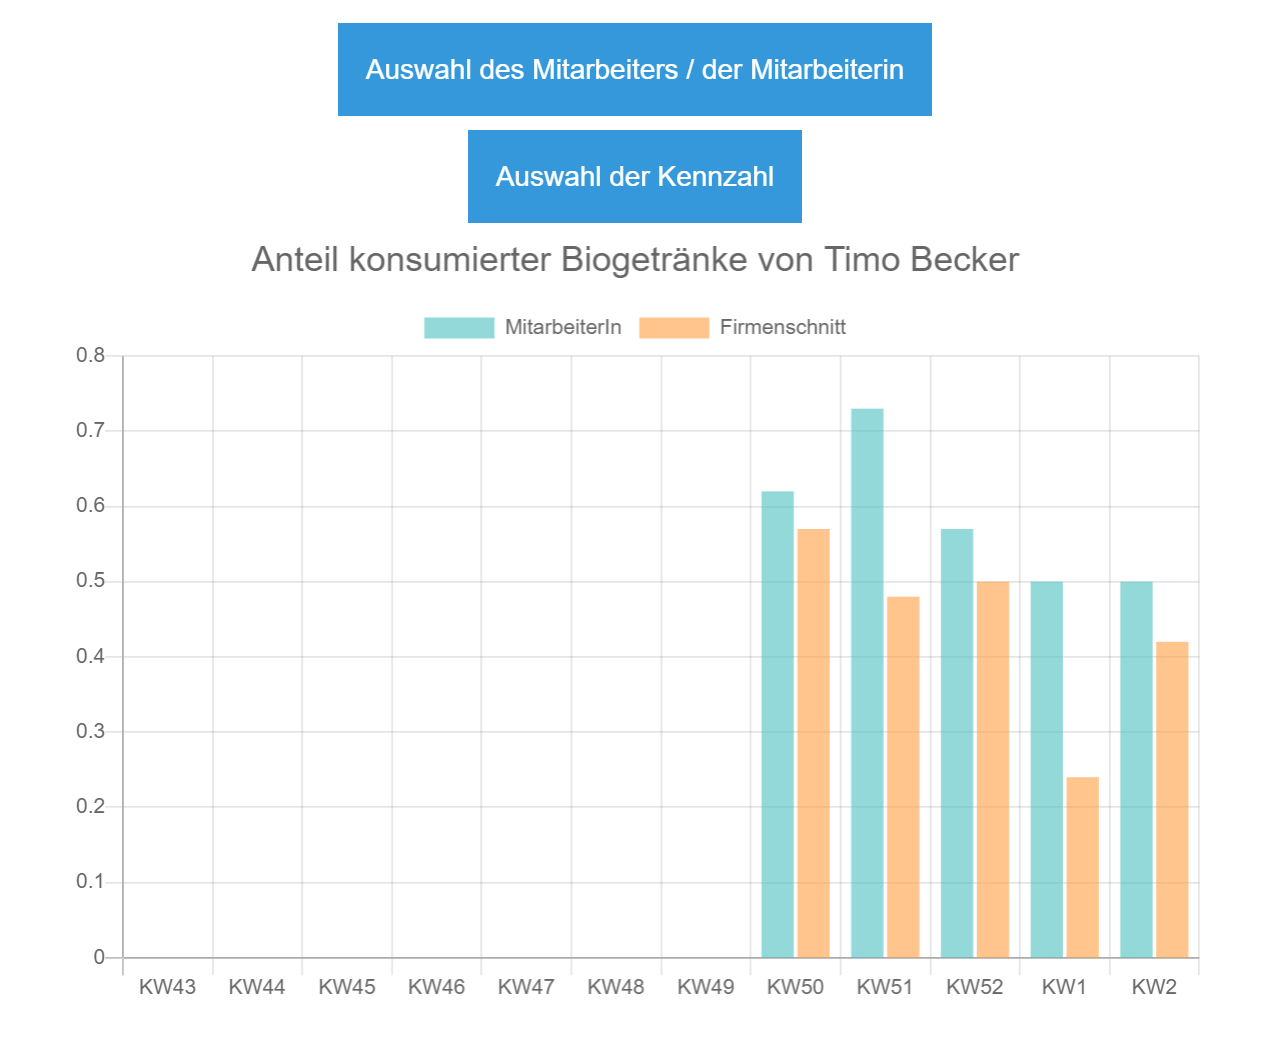
\includegraphics[width=0.7\textwidth]{Picture1.PNG}
\caption{nur Daten von 5 Wochen verfügbar.}
\end{figure}

\paragraph{ii. Was passiert wenn Logfiles von mehr als 12 Wochen vorliegen?}
In diesem Fall werden auf dem Bottle Webserver nur die Daten der letzten 12 Logfiles im JSON Format abgelegt.

\paragraph{iii. Was passiert wenn ein Mitarbeiter keinen Kaffee trinkt?}
In diesem Fall taucht der Mitarbeiter zwar nicht in den Logfiles des Kaffeeautomaten auf, jedoch ist er in der Mitarbeiterdatenbank angelegt und wird deshalb trotzdem in der Tabelle und auch im letzten Diagramm angezeigt.

\paragraph{iv. Kann ein Mitarbeiter die Daten der Kollegen einsehen?}
Ja, dies ist explizit von uns absichtlich so umgesetzt. Sowohl in der Tabelle als auch im letzten Chart des Plugins sind die Namen der Mitarbeiter und die zugehörigen Daten für alle anderen sichtbar.



\end{document}
